% !TeX root = ../../../book.tex

\subsection{函数复合}

\begin{multicols}{2}
    \begin{center}
        {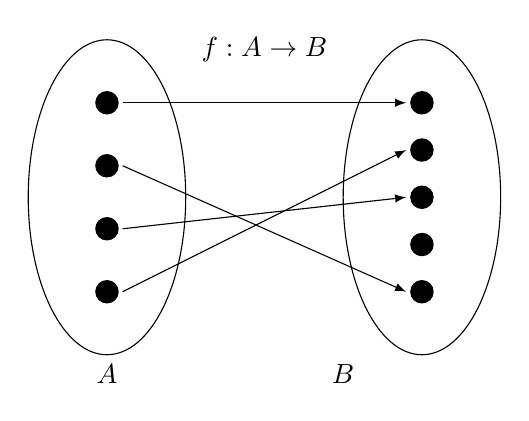
\begin{tikzpicture}[scale=1]
            \foreach \x in {0,...,4}
            {
                \node at (4, -\x*0.6)[circle,fill,inner sep=3pt]{};
            }
            \draw (4,-1.2) ellipse (1 and 2);
    
            \foreach \x in {0,...,3}
            {
                \node at (0, -\x*0.8)[circle,fill,inner sep=3pt]{};
            }
            \draw (0,-1.2) ellipse (1 and 2);
    
            \draw[-latex] (0.2,-0.0) -- (3.8,0.0); 
            \draw[-latex] (0.2,-0.8) -- (3.8,-2.4); 
            \draw[-latex] (0.2,-1.6) -- (3.8,-1.2); 
            \draw[-latex] (0.2,-2.4) -- (3.8,-0.6); 
            
            \node[below] at (0, -3.2){$A$};
            \node[below] at (3, -3.2){$B$};
            \node[above] at (2, 0.4){$f:A \to B$};
        \end{tikzpicture}}
    \end{center}

    \begin{center}
        {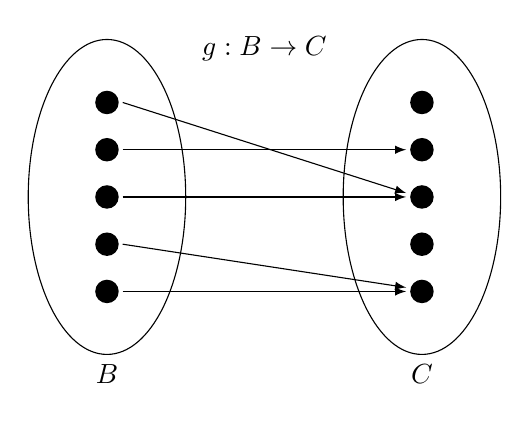
\begin{tikzpicture}[scale=1]
            \foreach \x in  {0,...,4}
            {
                \node at (4, -\x*0.6)[circle,fill,inner sep=3pt]{};
            }
            \draw (4,-1.2) ellipse (1 and 2);
    
            \foreach \x in  {0,...,4}
            {
                \node at (0, -\x*0.6)[circle,fill,inner sep=3pt]{};
            }
            \draw (0,-1.2) ellipse (1 and 2);
    
            \draw[-latex] (0.2,-0.0) -- (3.8,-1.15); 
            \draw[-latex] (0.2,-0.6) -- (3.8,-0.6); 
            \draw[-latex] (0.2,-1.2) -- (3.8,-1.2); 
            \draw[-latex] (0.2,-1.8) -- (3.8,-2.35); 
            \draw[-latex] (0.2,-2.4) -- (3.8,-2.4); 
            
            \node[below] at (0, -3.2){$B$};
            \node[below] at (4, -3.2){$C$};
            \node[above] at (2, 0.4){$g:B \to C$};
        \end{tikzpicture}}
    \end{center}
\end{multicols}


\begin{center}
    {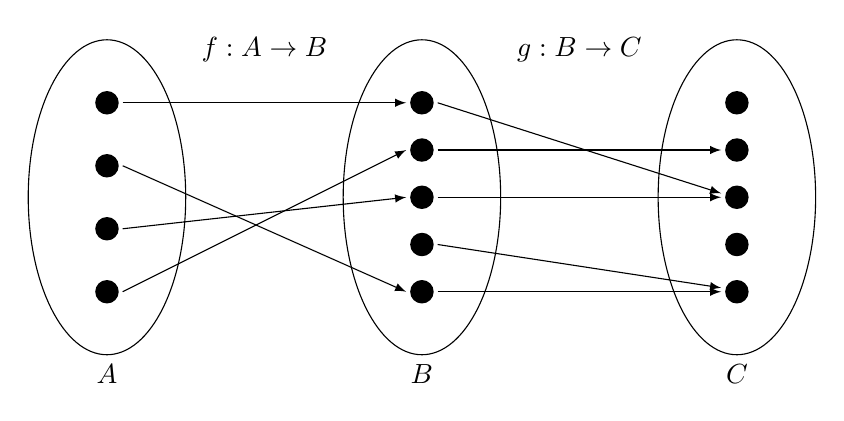
\begin{tikzpicture}[scale=1]
        \foreach \x in {0,...,3}
        {
            \node at (0, -\x*0.8)[circle,fill,inner sep=3pt]{};
        }
        \draw (0,-1.2) ellipse (1 and 2);

        \foreach \x in {0,...,4}
        {
            \node at (4, -\x*0.6)[circle,fill,inner sep=3pt]{};
        }
        \draw (4,-1.2) ellipse (1 and 2);

        \foreach \x in  {0,...,4}
        {
            \node at (8, -\x*0.6)[circle,fill,inner sep=3pt]{};
        }
        \draw (8,-1.2) ellipse (1 and 2);

        \draw[-latex] (0.2,-0.0) -- (3.8,0.0); 
        \draw[-latex] (0.2,-0.8) -- (3.8,-2.4); 
        \draw[-latex] (0.2,-1.6) -- (3.8,-1.2); 
        \draw[-latex] (0.2,-2.4) -- (3.8,-0.6); 

        \draw[-latex] (4.2,-0.0) -- (7.8,-1.15); 
        \draw[-latex] (4.2,-0.6) -- (7.8,-0.6); 
        \draw[-latex] (4.2,-1.2) -- (7.8,-1.2); 
        \draw[-latex] (4.2,-1.8) -- (7.8,-2.35); 
        \draw[-latex] (4.2,-2.4) -- (7.8,-2.4); 
        
        \node[below] at (0, -3.2){$A$};
        \node[below] at (4, -3.2){$B$};
        \node[below] at (8, -3.2){$C$};
        \node[above] at (2, 0.4){$f:A \to B$};
        \node[above] at (6, 0.4){$g:B \to C$};
    \end{tikzpicture}}
\end{center}

\begin{center}
    {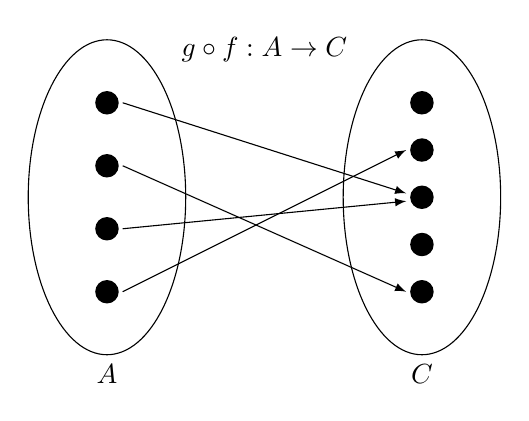
\begin{tikzpicture}[scale=1]
        \foreach \x in {0,...,4}
        {
            \node at (4, -\x*0.6)[circle,fill,inner sep=3pt]{};
        }
        \draw (4,-1.2) ellipse (1 and 2);

        \foreach \x in {0,...,3}
        {
            \node at (0, -\x*0.8)[circle,fill,inner sep=3pt]{};
        }
        \draw (0,-1.2) ellipse (1 and 2);

        \draw[-latex] (0.2,-0.0) -- (3.8,-1.15); 
        \draw[-latex] (0.2,-0.8) -- (3.8,-2.4); 
        \draw[-latex] (0.2,-1.6) -- (3.8,-1.25); 
        \draw[-latex] (0.2,-2.4) -- (3.8,-0.6); 
        
        \node[below] at (0, -3.2){$A$};
        \node[below] at (4, -3.2){$C$};
        \node[above] at (2, 0.4){$g \circ f:A \to C$};
    \end{tikzpicture}}
\end{center}